\mychapter{Introdução}
\label{Cap:Introducao}

O setor industrial brasileiro, responsável por cerca de 20\% do PIB e 70\% das exportações \cite{cni2024}, enfrenta desafios constantes, sendo crucial para a economia nacional. A necessidade de inovação e investimentos em tecnologia apresenta ser um dos pilares da evolução do setor industrial brasileiro \cite{produtividadeindustria}. Nesse cenário, o \textit{software} de reconciliação de dados \textit{online}, denominado DRD, foi desenvolvido como uma proposta inovadora para aprimorar a qualidade e confiabilidade dos dados nos processos industriais, enquanto oferta uma interface gráfica de fácil uso e com funcionalidades de uma API (\textit{Application Programming Interface}) que permite adaptações para atender à diferentes aplicações industriais.

A precisão dos dados de processo nas indústrias químicas/petroquímicas desempenha um papel crucial no desempenho operacional e nos ganhos financeiros provenientes da utilização de diversos \textit{softwares} para monitoramento de processos, otimização \textit{online} e controle \cite{datarecshakar}. Entretanto, as medições realizadas na planta frequentemente apresentam imprecisões causadas por erros aleatórios ou sistemáticos que comprometem o modelo de processo utilizado para otimização e controle. E, para resolver problemas dessa natureza, foi desenvolvida a área de conhecimento da reconciliação de dados que faz uso de equações de processos, relações de equilíbrio e leis de conservação de massa e energia \cite{reformulationdatarecon}. De todos os possíveis métodos a serem aplicados no \textit{software} DRD, o escolhido foi o de minimização de funções multivariáveis utilizando o método dos multiplicadores de Lagrange. 

O desenvolvimento \textit{web} tem experimentado um notável crescimento na última década \cite{webusage}, e há vantagens distintas em um ambiente de \textit{software web} que não são tão prontamente acessíveis em outras áreas. As características destacáveis incluem a implementação de um sistema de API \cite{apirest}, possibilitando a interoperabilidade eficiente entre diferentes sistemas, o acesso remoto de qualquer local, a transposição fluida de ambiente de um local para outro, a facilidade inerente de manuseio \cite{apiimportance} e a capacidade natural de construção de sistemas com alta acessibilidade à indivíduos com imparidade visual. Esses atributos fazem do ambiente \textit{web} uma escolha propícia para o desenvolvimento deste sistema, proporcionando uma experiência aprimorada em comparação com alternativas menos dinâmicas, desta forma saciando uma falta do mercado como também explorando uma área não investida atualmente.

Dessa forma, é notável a necessidade de uma ferramenta que possa unificar esses dois campos, como o \textit{software} DRD. Ao integrar a teoria da reconciliação de dados com as modernas técnicas de desenvolvimento de \textit{software}, o DRD representa um avanço significativo na busca por soluções inovadoras e eficazes para os desafios enfrentados pelas indústrias. Além disso, ao aproveitar as vantagens do ambiente \textit{web}, o DRD oferece uma plataforma flexível e adaptável, capaz de atender às demandas específicas de diferentes setores industriais, promovendo assim a excelência operacional e impulsionando o desenvolvimento tecnológico do Brasil \cite{industry4status}.

\section{Objetivos}
\subsection{\textit{Objetivo geral}}

Desenvolver e implementar um \textit{software web} para a reconciliação dos dados oriundos de processos industriais, por meio do método de multiplicadores de Lagrange, visando aumentar a qualidade e a confiabilidade das informações para a análise e a tomada de decisão.

\subsection{\textit{Objetivos específicos}}

Além de buscar alcançar o objetivo principal de desenvolver uma ferramenta \textit{online} de reconciliação de dados, realizações secundárias serão contempladas, as quais serão úteis para cumprimento do objetivo alvo. Esses objetivos gerais são descritos a seguir: 

\begin{itemize}
    \item Pesquisar a respeito do estado da arte sobre as principais técnicas e ferramentas de validação, limpeza e reconciliação de dados. 
    \item Analisar e compreender as metodologias e algoritmos existentes na área de reconciliação de dados, destacando suas aplicações, vantagens e limitações. A pesquisa de estado da arte é crucial para identificar as tendências mais recentes, as melhores práticas e as lacunas existentes, proporcionando uma base sólida para o desenvolvimento da ferramenta \textit{online}.
    \item Selecionar e adaptar as tecnologias adequadas para a implementação da ferramenta \textit{online} de reconciliação de dados. Isso envolverá a avaliação de linguagens de programação, \textit{frameworks} e plataformas que melhor se adéquem aos requisitos específicos da aplicação, considerando aspectos como eficiência, escalabilidade e segurança.
    \item Projetar a arquitetura da ferramenta, delineando os componentes principais, a interação entre eles e a lógica de funcionamento. A clareza na definição da arquitetura será essencial para garantir a eficácia operacional da ferramenta, bem como para facilitar futuras atualizações e expansões.
    \item Desenvolver a ferramenta \textit{online} de reconciliação de dados, implementando os algoritmos e funcionalidades identificados na pesquisa de estado da arte. Durante essa fase, é crucial garantir a usabilidade, a integridade dos dados e a eficiência do sistema, atendendo aos padrões de qualidade e indicadores de desempenho esperados.
    \item Realizar testes abrangentes para validar a eficácia e confiabilidade da ferramenta. Isso incluirá testes de integração, testes de segurança e simulações de casos práticos para verificar a capacidade da ferramenta em lidar com diferentes cenários e volumes de dados.   
    \item Elaborar uma documentação completa, abrangendo desde o processo de desenvolvimento até as instruções de uso da ferramenta. Uma documentação completa, acessível, clara e objetiva será essencial para facilitar a compreensão, manutenção e futuras implementações relacionadas à ferramenta de reconciliação de dados.
\end{itemize}

\section{Estado da Arte}

Em meio ao processo de elaboração do trabalho de conclusão de curso, um aspecto fundamental que merece destaque é a investigação das tendências tecnológicas emergentes nas áreas relevantes para o estudo. Essa pesquisa não apenas fornece uma visão abrangente do cenário atual, mas também ajuda a identificar oportunidades para inovação e melhoria.

As tendências tecnológicas são indicadores poderosos do progresso em qualquer campo de estudo e podem ser representadas tanto na área comercial direta, como na indústria química, nas áreas adjacentes, como em conceitos de contabilidade, além de pesquisas cientificas. Elas refletem os avanços mais recentes e as direções futuras que a tecnologia pode tomar. Portanto, é essencial estar ciente dessas tendências ao realizar qualquer pesquisa acadêmica ou científica.

\subsection{Aplicação na Indústria Química}

No contexto da indústria química, há várias empresas com soluções similares à proposta neste trabalho, e a investigação das tendências tecnológicas emergentes é um aspecto crucial durante o processo de elaboração dessa ferramenta (DRD). 

\subsubsection{RECON}

A ChemPlant Technology, s.r.o, fundada em 1991 é uma empresa situada na Republica Checa, especializada em fornecer soluções tecnológicas avançadas para indústrias de processos (principalmente, processos químico, petróleo e gás, geração e distribuição de energia) \cite{reconset}. Uma de suas inovações mais notáveis é a ferramenta de reconciliação de dados chamada RECON. Esta ferramenta é fundamentada nos sólidos princípios físicos de balanço de massa e energia, um \textit{software} interativo abrangente que oferece uma plataforma robusta para modelagem de complexas plantas industriais químicas e energéticas. Ele realiza uma variedade de cálculos, incluindo balanceamento de massa, energia e momento, bem como cálculos termodinâmicos. O principal objetivo da solução é validar dados que já foram obtidos de processos operacionais. No entanto, a ferramenta, exposta na Figura \ref{fig:RECONSET} também pode ser utilizada para simular o comportamento da planta sob diferentes condições.

\begin{figure}[htbp!] 
    \begin{center}
        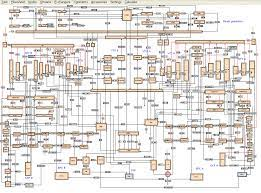
\includegraphics[width=0.75\textwidth]{figuras/RECONSET.jpg}
        \caption{Tela Principal da ferramenta RECONSET.}
        \vspace{6mm}
        \label{fig:RECONSET}
    \end{center} 
\end{figure}

O \textit{software} é orientado para PC e possui uma interface de usuário gráfica interativa, tornando-o fácil de usar. Os usuários definem problemas (ou tarefas) interativamente por meio desta interface. O RECON é capaz de equilibrar materiais e energia de componentes únicos ou múltiplos de sistemas complexos, seja em estado estacionário ou instável (dinâmico), com ou sem reações químicas (balanceamento de reatores). Além disso, ele pode realizar balanceamento de momento com base em cálculos hidráulicos de vazão em sistemas de dutos. O RECON reconcilia vazões medidas, concentrações, temperaturas e outras variáveis de processo, e calcula variáveis não medidas. Para definir um problema (ou tarefa), os usuários geralmente criam um fluxograma de processo e definem variáveis de processo, como taxas de fluxo, temperaturas, pressões, etc. O fluxograma inclui nós, fluxos de massa e energia, e trocadores de calor. Se necessário, os usuários também podem complementar (ou até mesmo substituir) o modelo de balanceamento com suas próprias equações.

\subsubsection{BILCO}

CASPEO é uma empresa francesa fundada em 2004, especializada em engenharia de processos e soluções tecnológicas. Originada do 
Departamento de Pesquisas Geológicas e Minerais da França. Ela foi criada para oferecer à indústria de mineração métodos e ferramentas computacionais resultantes de anos de pesquisa e tornou-se uma referência na indústria de processamento mineral, atendendo a vários mercados, como mineração e metalurgia, processamento de biomassa e alimentos, tratamento de resíduos sólidos e outras indústrias de processamento \cite{bilco}.

Uma das suas inovações é o \textit{software} de reconciliação de dados BILCO, projetado para derivar um balanço de material coerente e total a partir de todos os dados disponíveis (medições, análises, estimativas) para todas as correntes de processo. Ele é uma ferramenta poderosa que permite aos usuários reconciliar dados de qualquer planta de processamento, a Figura \ref{fig:BILCO}, demonstra a tela inicial do \textit{software}.

\begin{figure}[htbp!] 
    \begin{center}
        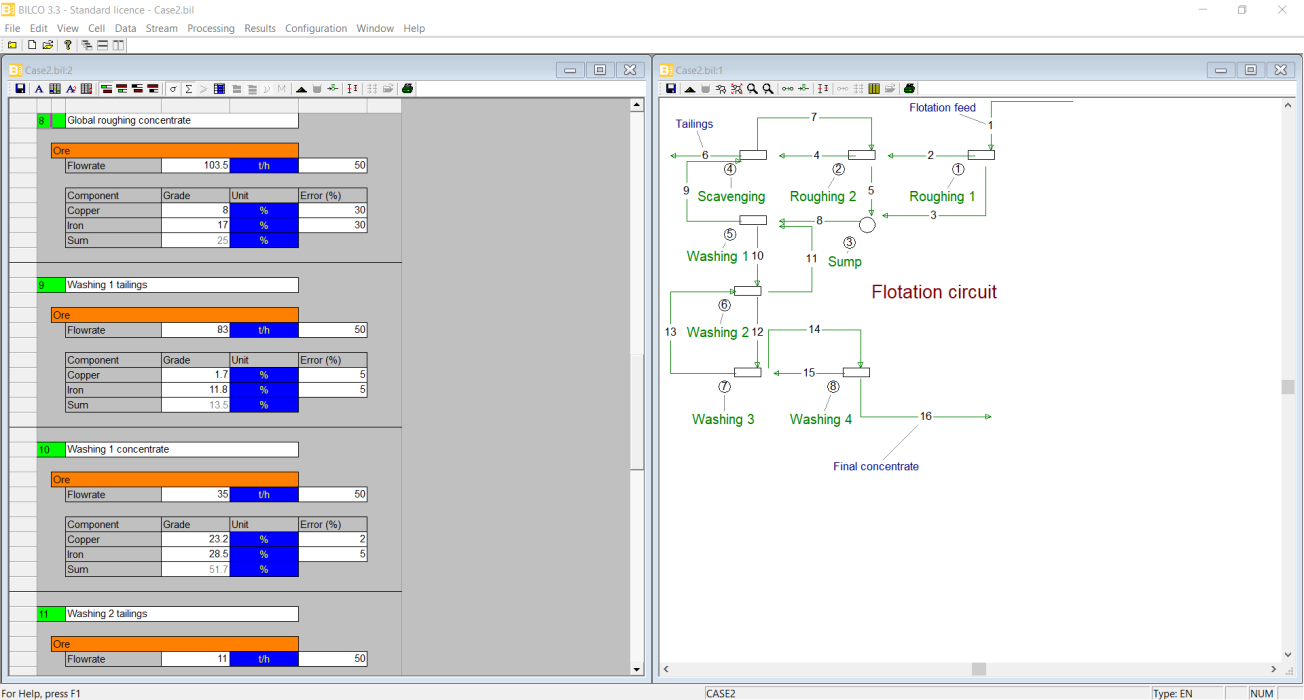
\includegraphics[width=0.75\textwidth]{figuras/BILCOCASPEOP.png}
        \caption{Tela Principal da ferramenta BILCO.}
        \vspace{6mm}
        \label{fig:BILCO}
    \end{center} 
\end{figure}

Ele tem a capacidade de se incorporar à duas outras ferramentas facilmente, no caso, à um simulador de processos, denominado USIM PAC e à um \textit{software} de contabilidade metalúrgica, INVETEO; e, dessa forma, fornece cálculos de balanço precisos e gera um conjunto de estimadores coerentes que estão em conformidades com as restrições da lei de conservação de energia, além de calcular seus erros relativos. Ele também é capaz de determinar, em quantidade e qualidade, a composição de cada corrente de processo. É um dos poucos \textit{softwares} de balanço de massa capaz de calcular toda a composição da corrente (taxas de fluxo, classes de tamanho, tipos de partículas, massa molar, etc.) em um único cálculo.

Essa solução também oferece uma única interface para gerenciar todo o processo. Consiste numa interface gráfica fácil de usar, tornando-a acessível tanto para novos usuários quanto para os mais experientes. Uma das características mais úteis do BILCO é a possibilidade de exportar os resultados para o Excel, permitindo uma análise mais profunda dos dados. Ele fornece resultados detalhados, incluindo uma planilha de comparação e uma planilha global, para uma visão completa do balanço de material.

\subsubsection{PIMSOFT}

Shorou International é uma empresa dos Emirados Árabes Unidos, que oferece soluções especializadas e serviços de engenharia com foco em automação avançada e gestão de ativos para todas as principais indústrias, com ênfase especial nos setores de petróleo, gás, utilidade e energia \cite{pimsoft}.

Uma das suas soluções é o Sistema OSIsoft PI, uma plataforma que coleta, historiza e analisa grandes quantidades de dados de séries temporais, de alta fidelidade, de várias fontes de dados e em diferentes formados. Esses dados são disponibilizados para usuários e sistemas em diversos setores de negócios. As implementações do sistema PI aproveitam o poder dos dados operacionais para gerar previsões que aumentam a consciência situacional e desencadeiam decisões bem planejadas, ajudando as empresas líderes a alcançar maiores melhorias operacionais e inovações revolucionárias em seus respectivos campos. 

E um complemento desse sistema, é o PIMSOFT SigmaFine que é um \textit{software} de verificações e balanços que utiliza princípios de conservação, estatísticas, padrões de engenharia e cálculos para monitorar e montar dados de plantas industriais. SigmaFine gera módulos coerentes, confiáveis e utilizáveis, prontos para negócios.

\subsection{Aplicação na Contabilidade}

Paralelamente à disciplina de Reconciliação de Dados na área industrial química, há uma outra área na qual investe bastante nesse campo, a de soluções contábeis. E a investigação das tendências tecnológicas emergentes é um aspecto crucial durante o processo de desenvolvimento de uma solução mais dinâmica e que consegue resolver problemas já solucionados por outras áreas da ciência.

\subsubsection{FloQast}

FloQast é uma empresa fundada em 2013, que possui uma plataforma  de contabilidade operacional baseada na nuvem, com foco em automação e gestão para uso por contadores. Uma das suas soluções é uma ferramenta de reconciliação de dados nomeada FloQast Reconciliation Management, uma solução avançada de automação de fluxo de trabalho para fornecer gerenciamento de reconciliação de contas de ponta a ponta \cite{floqast}.

Isso aumenta a velocidade e a precisão financeira do fechamento financeiro, ao mesmo tempo que gerencia o risco de declaração incorreta. Esse \textit{software} permite que controladores e suas equipes automatizem e gerenciem o processo de reconciliação de ponta a ponta, com uma solução centralizada confiável por contadores e auditores em todo o mundo.

\subsubsection{Aspen}

AspenTech, uma empresa fundada em 1981, a partir do Projeto ASPEN - uma pesquisa conjunta entre o MIT (Instituto de Tecnologia de Massachusetts) e o Departamento de Energia dos EUA na qual desenvolveu a primeira tecnologia de modelagem e simulação baseada em computador para a indústria química. Hoje, mais de 40 anos depois, com mais de 3700 funcionários e 60 localidades em todo o mundo, a empresa tem seu foco em soluções industriais, ao mesmo tempo em que enfrenta diretamente a sustentabilidade, com foco na eficiência dos recursos, transição energética, descarbonização e redução de resíduos \cite{aspen}.

Uma das suas ferramentas que utiliza soluções similares às do trabalho de conclusão de curso é a ferramenta AURA (Aspen Unified Reconciliation Accounting) uma solução que ajuda a reduzir perdas de material e aumentar margens por meio de um equilíbrio eficiente de massa e volume. Capacitando as partes interessadas a tomar melhores decisões com base em dados de produção validados e reconciliados. Sua arquitetura escalável reduz o custo total de propriedade com opções rápidas de implantação na nuvem e fácil implementação e manutenção do modelo. A precisão da reconciliação é aumentada pelo \textit{Smart Solver} proprietário que resolve automaticamente os erros de densidade medidos em laboratório. O \textit{software} também ajuda a atingir metas de redução de emissões ao automatizar o rastreamento, monitoramento e relatórios de emissões de gases de efeito estufa e intensidade de carbono do produto. Além disso, permite fechar o balanço mais rapidamente com fluxos de trabalho intuitivos, interpretação fácil dos resultados com visualização avançada e relatórios dinâmicos poderosos.

\subsection{Pesquisas Sendo Desenvolvidas}

Como o objetivo do DRD é ser uma ferramenta que consegue recolher avanços tecnológicos de cada área, é de suma importância não só estar ciente e alinhado às tendências da própria área de aplicação, como das adjacentes, mas também estar alinhado às pesquisas da área de reconciliação de dados computacional. 

\subsubsection{Controle e Supervisão de Processamento Mineral}

A pesquisa apresentada por Daniel Hoduin, \cite{danielhoduin}, dá  ênfase às restrições de conservação de massa e energia, que são usadas como base para o projeto de estratégias de medição, atualização do valor medido por técnicas de filtragem de erros de medição e estimativa de variáveis de processo não medidas. Como as principais variáveis numa unidade de processamento mineral são geralmente vazões e concentrações, a sua reconciliação com as leis de conservação de massa é central para as técnicas discutidas. São propostas ferramentas para três tipos diferentes de regimes operacionais: regime estacionário, estacionário e dinâmico. Esses métodos de reconciliação são baseados nos mínimos quadrados usuais e nas técnicas de filtragem de Kalman.

\subsubsection{Balanços de Materiais em Rede de Distribuição de Gás}

O desenvolvimento feito pelos pesquisadores Jesús David Badillo Herrera, Arlex Chaves e José Augusto Fuentes Osorio \cite{balancecontrol}, oferece uma solução prática para lidar com os desafios apresentados por erros em sistemas de distribuição de gás natural. Ao combinar técnicas numéricas e estatísticas, como a Reconciliação de Dados (DR) e a Detecção de Erros Brutos (GED), a ferramenta visa aprimorar a precisão das medições, garantir conformidade com as leis de conservação de massa e identificar e corrigir erros grosseiros. A validação da ferramenta por meio de problemas da literatura e sua aplicação a uma rede de distribuição real demonstram sua eficácia em fornecer resultados reconciliados precisos. Essa ferramenta tem o potencial de aprimorar a eficiência e confiabilidade dos processos de distribuição de gás natural, minimizando perdas de receita e complicações legais.

\section{Justificativa}

A construção do projeto de \textit{software} DRD é fundamentada na urgente necessidade de soluções inovadoras para superar os desafios do setor industrial brasileiro. Este setor é essencial para a economia do país, apesar dos constantes obstáculos que enfrenta. Destaca-se, portanto, a importância da inovação e do investimento em tecnologia como motores do seu desenvolvimento.

Além disso, a escolha de desenvolver o \textit{software} como uma aplicação \textit{web} aproveita as vantagens desse ambiente, incluindo interoperabilidade eficiente entre sistemas, acesso remoto, facilidade de uso e alta acessibilidade para indivíduos com necessidades especiais, não apenas atendendo às demandas do mercado atual, mas também representa uma inovação ao explorar uma área ainda não totalmente investida. A importância desse projeto é ainda mais destacada pela análise das tendências tecnológicas emergentes em áreas relevantes, como a indústria química. Empresas e pesquisadores estão desenvolvendo ferramentas e técnicas semelhantes, demonstrando a relevância e a demanda por soluções que otimizem a reconciliação de dados e garantam a precisão das informações.

Portanto, a solução visa preencher uma lacuna no mercado brasileiro, oferecendo uma ferramenta inovadora e eficaz para reconciliação de dados industriais. Ao integrar teoria e prática, o DRD tem o potencial de impulsionar a excelência operacional e promover o desenvolvimento tecnológico do país, contribuindo para o aumento da competitividade das indústrias brasileiras no cenário global.

O trabalho aqui apresentado é organizado da seguinte forma: no Capítulo 1 é feita a introdução do trabalho, apresentando o problema e seu contexto, citando sua solução de forma delimitada e com os objetivos principal e secundário de forma clara, e fazendo uma revisão bibliográfica sobre ferramentas que possuem alguma semelhança com a ferramenta aqui proposta; no Capítulo 2 é apresentado o referencial teórico que trás definições, descrições e detalhes sobre as principais teorias que embasam a solução proposta; o Capítulo 3 descreve como os diferentes métodos e técnicas corroboram para o êxito da solução aqui planejada e também é apresentado um cronograma de atividades, por meio do diagrama Gantt, que será útil para o organização e gerenciamento do desenvolvimento das etapas para realização da solução aqui proposta quanto no trabalho de conclusão de curso 2; por fim, no Capítulo 4 são realizadas considerações finais acerca do aprendizado com a realização deste trabalho, acerca das reflexões e ponderações sobre as expectativas de resultados para o desenvolvimento futuro do TCC2 e também sobre as contribuições desta obra.